% !TEX root =single_chapter_dalek.tex
\chapter{Automatic fitting of optical Type Ia Supernova spectra - the DALEK project}
\label{chap:dalek}

The last chapters (Chapters \ref{chap:sn1572_starg, chap:sn1572_hires, chap:sn1006_flames} were dedicated to the hunt for donor stars and did not use the measurements from the \snia-phenomenon itself. In this chapter we will describe the extraction of yields and energies from optical spectra. 

The two main sources of information in spectra, are the spectra themselves as well as their time evolution. There have been a few attempts to extract the details of the stellar explosions from one or two of these sources. All of them employ the technique of fitting the spectra using synthetic spectra. One of the main parts is the radiative transfer program that creates the synthetic spectra. There are several different radiative transfer-codes in the community. 


\cite{2000PhDT.........6F} wrote a very simple radiative transfer code called \synow. \synow is a highly parametrized code and thus is mainly used for line identification rather than actual fitting of supernova spectra. It runs 
The main code (henceforth \mlc) used in this work is an evolved code of  \cite{1993A&A...279..447M, 2000A&A...363..705M}. Compared to the \synow-code the \mlc-code calculates a radiative equlibirum tepmerature and uses this to compute internally consistent ionization ratios. In addition \mlc takes electron scattering into account as well as allowing for photon branching. 


Codes such as PHOENIX\cite{1999JCoAM.109...41H}, SEDONA \cite{2006ApJ...651..366K} and ARTIS \cite{2009MNRAS.398.1809K} are powerful 3D radiative transfer codes. They are the most "physical" codes available but take hours on supercomputers to produce spectra. These codes, however, are not feasible for fitting observed spectra as they take too long for each iteration. 

The main aim of this work is to automatically fit the torrent of observed spectra expected from the current and next generation of supernova searches. We opted to use the \mlc-code as it provides a good compromise between speed and "realism".

In section \ref{sec:mlc_intro}we will introduce a the inner-workings of the \mlc-code.  We will discuss the properties of the search space in \ref{sec:searchspace} and will introduce our optimisation strategies in \ref{sec:optimisation_strategies}. Finally we will conclude and give an outlook over future work for this unfinished project in section \ref{sec:dalek_conclusion}.

\section{The \mlc-Code}

The supernova can be divided in two different phases: the photospheric phase and the nebular phase. The \mlc-code only models the photospheric phase.
In this photospheric phase the supernova is treated like a sharp photosphere emitting a black-body spectrum with a fast moving layer of ejecta above that. 

There are many physical processes in radiative transfer. Of those the Bound-free opacity has the biggest contribution to the final spectrum. In addition, Thompson scattering is thought to have an important effect in redistributing the flux. As \mlc is required to run fast only Bound-Free opacity as well as Thompson scattering is implemented in the code.

Unlike stellar atmospheres in supernova ejecta one needs to consider the photon's doppler shift in relation to the surrounding medium. One major assumption that the code makes is that of the Sobolev approximation.  This means that at the interaction between photon and line resonance happens only at one specific point (thus disregarding any broadening effects to the line). For example a photon in free flight from the photosphere will be able to interact with resonance lines of lower and lower frequencies. The Sobolev approximation makes the code relatively fast 

Another assumption that \mlc makes is that the ejecta is in homologous expansion. This means that the velocity is a linear function of the radius:
\[
	v=  r / t.
\]

Combining both the Sobolev approximation with the assumption of homologous expansion yields this relatively simple formulat for line opacities:
\[
\tau_{ul} = \frac{\pi e^2}{m_e c}\, f \lambda t_{\rm exp} n_l\, \left(1 - \frac{g_l n_u}{g_u n_l}\right), 
\]
where $\tau_{ul}$ denotes the opacity going from the u-state to the l-state, $e$ is the electron charge, $m_e$ is the electron mass, f is the oscilator strength of the line, $\lambda$ denotes the wavelength, $t_exp$ the time since explosion, $n_x$ the number of atoms in the state x and $g_x$ is the statistical weight of the state x.
Both homologous expansion and Sobolev approximation have their caveats. In the case of homologous expansion it is thought to be a very good approximations after the first few minutes after the explosion. The main caveat for Sobolev approximation is that a line is not a delta-function, as assumed in the Sobolev approximation. If too strong bound-bound lines are close in frequency space it can lead to the first line shielding the second line. In summary for fast supernova fitting both approximations seem to still allow for a relatively well fitting spectrum.

We have discussed the propagation of the photons in the plasma but have not discussed the state of the plasma yet. The simplest assumption for the state one can make is local thermodynamic equilibrium. In this case the Boltzmann formula describes the level populations in a single ion:
\[
\frac{n_j}{n_{\rm ground}} = \frac{g_j}{g_{\rm ground}}\,e^{-(\epsilon_j - \epsilon_{\rm ground})/kT}
\]
Similarly we can calculate the ionization state using the Saha-equation:
\[
	\frac{N_j}{N_{j+1}} = n_e \frac{U_j(T)}{U_{j+1}(T)}\,C_I T^{-3/2} e^{\chi/kT},
\]
where $U_j$ is the partition function and $C_I$ is a constant. As the ionization likelyhood depends on the internal electronic state of the atom the partition function sums up over the different states:
\[
U_j = \sum_i g_{i,j} e^{-\frac{E_{i,j}}{kT}},
\]
where i describes the excitation states and j the ionization states. The other symbols have their usual meaning. 
The sum normally diverges slowly so one in practice just sums up until a highly excited state.

The \mlc\ uses the so called \textit{nebular approximation} which will calculate the excitation and ionization state of the SNe at nearly LTE cost. In this nebular approximation they introduce a dilution factor $W$. This is a purely geometrical factor. Treating the photosphere as a point source the factor would result in $W=1/r^2$ with r being the distance from the center. As the photosphere is expanded the dilution factor has a slightly more complex formula. An important point to note is that purely theoretical at the photosphere the dilution factor is 0.5.

The mean intensity for the supernova at a specific zone is given as:
\[
J = W B(T_R),
\]
where $T_R$ is the radiative temperature. The radiative temperature is estimated in the \mlc\ by matching the mean frequency of $B(T_R)$ with the mean frequency of the photon packets in the current zone (Wien approximation). W is chosen so that the frequency-integrated intensity matches the photon distribution. 

Using $W$ and $J$ one now can calculate the electronic and ionization states of the plasma:
\[
\frac{n_j}{n_{\rm ground}} = W \left( \frac{n_j}{n_{\rm ground}} \right) _{T_R}^{\rm LTE}
\]
and 
\[
\frac{N_j}{N_{j+1}n_e} = W \left( \frac{N_j}{N_{j+1}n_e} \right) _{T_R}^{\rm LTE}
\]


In the simplest case we can treat the ejecta as homogeneous in temperature and abundance. For now we will also assume a pure scattering line interaction. This means that the photon is absorbed at a resonance frequency and then instantaneously reemitted with the same frequency into a random direction. This in in contrast to photon branching which we will discuss later. 

We assume a time since explosion $t_e$, a photospheric velocity \vph, \lbol and an abundance distribution for the chosen elements. W7 \citep{1984ApJ...286..644N} is used in the \mlc\ as a density structure.

The one dimensional model is divided into multiple zones that each have the same abundance but a different density. 
Using an initial guess of \teff\ for the photosphere, one can calculate the plasma condition in each shell. 

The Monte-Carlo simulation begins. A photon packet is emitted with a random frequency and a random angle drawn from a Blackbody distribution $B(T)$. Each photon packet contains the same energy (more photons per packet in the red than in the blue). 
An event optical depth is calculated from a uniform random distribution so that $\tau_{\rm event}=-ln(z); z \in (0,1]$.  
In the next step there are three possible outcomes. We calculate the length of the path ($s_e$) that the packet can travel freely before $\tau_{\rm event}$ is equal to the Thompson scattering opacity $\tau_{\rm event} = \sigma_{\rm T} n_e s_e$. Next we calculate the same path length for the lines $s_l$ using as a target opacity $\tau_e + \tau_{\rm line}$. 
If both paths are longer than the path to exit the current zone, then the photon exits the current zone and a new Monte Carlo process begins. 
If however $s_e$ is the shortest then Thompson scattering occurs and the photon is assigned a new direction and a new $\tau_{\rm event}$ is drawn and the process begins anew.

In the case of line scattering the excited atom can de-excite through many lines. \mlc randomly chooses a downward transition for the whole packet (taking the appropriate weights into account). The number of photons in the packet is adjusted to ensure that the energy is conserved in the comoving frame. 

There are two possibilities for the final fate of the photon. Either it is reabsorbed into the photosphere or is emitted from the supernova. 

When initializing the state of the plasma one assumes an initial guess for the photon temperature. The Monte-Carlo simulation is run and records each packet status at the mid-point of each shell. This information is used to calculate a new photospheric temperature and an updated plasma condition (level population and ionization). 
This procedure is repeated until the photospheric temperature converges. Once convergence is reached the actual Monte-Carlo simulation begins. 

The final spectrum is not calculated using the escaping packets. Instead we calculate the optical depths using and then calculate the emerging spectrum using the formal integral. 
This has the advantage of reducing noise in the spectrum due to Monte-Carlo noise and gives very good results. 

A more detailed description of the code can be found in  \cite{1993A&A...279..447M,2000A&A...363..705M}.




\section{Manually fitting a Type Ia supernova}

When fitting manually there are several features that help guide the direction of the fit. We will attempt to explain by using a spectrum of SN2002bo (cite?????) 10 days before maximum. In this section we will only talk about fits with no abundance stratification. Stephan Hachinger has kindly provided his manually obtained best fitting parameters ( for the supernova at this stage (see Figure \ref{fig:sn2002bo-10_bf}).
Directly measurable are the redshift of the supernova (and implied distance) and the time of the spectrum relative to maximum. We assume calculate the time since explosion assuming a rise time of 19.5 days.
The other parameters are initialized using empirical data. 

\begin{figure}[htbp] %  figure placement: here, top, bottom, or page
   \centering
   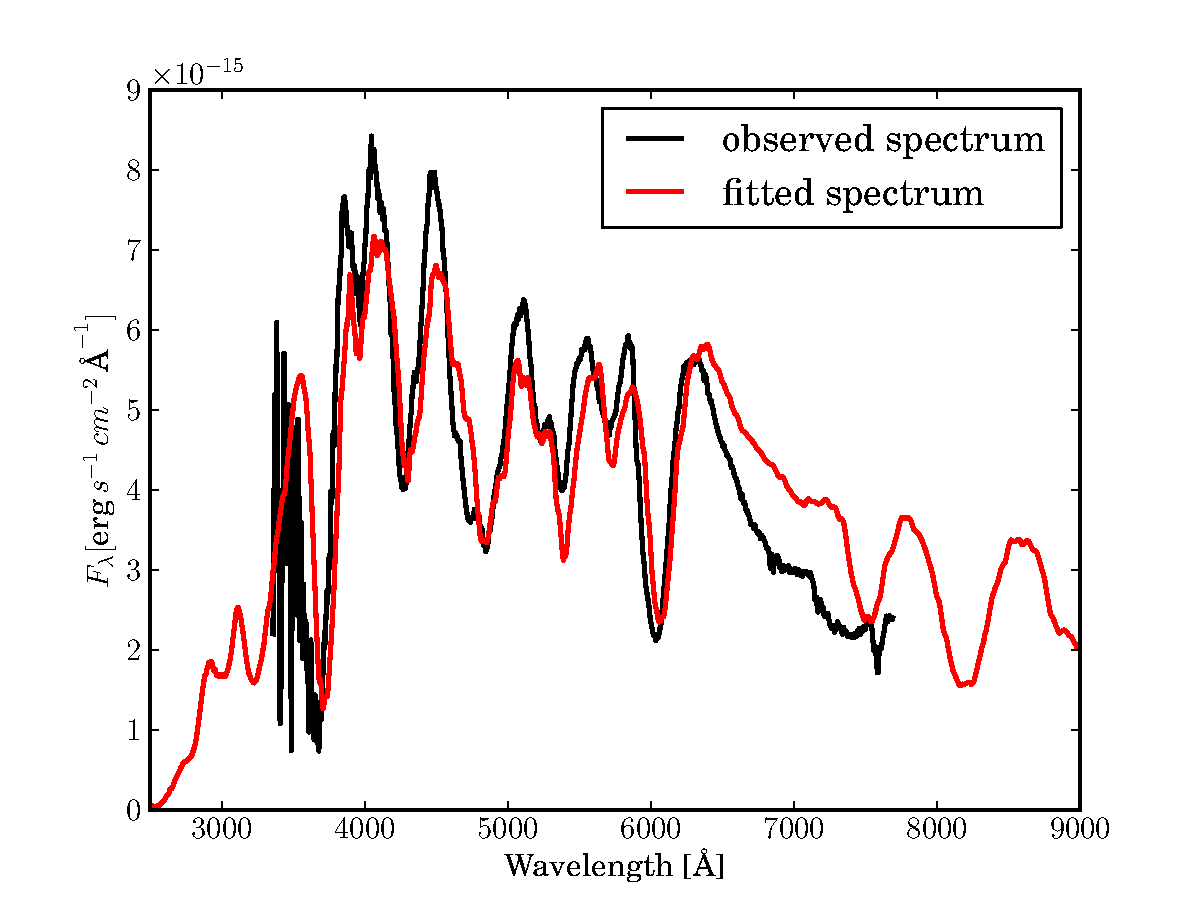
\includegraphics[width=\textwidth]{chapter_dalek/plots/bf2002bo-10.pdf} 
   \caption{example caption}
   \label{fig:sn2002bo-10_bf}
\end{figure}

The chosen fundamental parameters are $\loglbol=xx$, $\vph=xxx$. We have listed the non-zero abundances in Table \ref{tab:sn2002bo_perf_param}. 



The P-Cygni profiles of many features are easily visible. The Calcium line in the blue can be seen to be to blueshifted in relation to the model. This property is not unusual and is thought to come from high velocity component at the outer edge of the ejecta. The next major known discrepancy that can be seen is the excess of flux redwards of  $\approx 6200 \AA$.  This is a region that usually does not fit well as the underlying black body spectrum overestimates the flux in this region. When fitting manually often one tries to fit the depth the lines instead of the continuum.

There are three main parameters that have the most influence on the overall fit: Luminosity, photospheric velocity and abundance in iron group elements.

A large offset in \lum\ to the best fit paramater is easily visible as a large offset of the continuum (see Figure \ref{fig:sn2002bo_lum_offset}. Thus it is easy to constrain the parameter space in \lum\ initially. \lum\ also has influence on the temperature of the model through:
\[
L_{\rm bol} = 4\pi\sigma\, R^2\,T^4 = 4\pi\sigma\,\vph\,\texp.
\label{eq:lum_temp_relation}
\]

Velocity in astronomy is often measured using the doppler shift. In this case however it is hard to measure the photospheric velocity as lines are created at different depths and thus at different velocities. This smears out the line profiles which makes fitting velocities nearly impossible using this technique. 
The main impact of photospheric velocity is establishing the temperature given a luminosity. A model with a too high photospheric velocity will have expanded more than the real spectrum at that time and will be cooler. This results in a spectrum that is too luminous in the red and not luminous enough in the blue (see Figure \ref{fig:sn2002bo_vph_offset}). 
A secondary effect is that the ion population will be different to the actual supernova and the line spectrum differs.
\begin{figure}[htbp] %  figure placement: here, top, bottom, or page
   \centering
%   \includegraphics[width=2in]{replace} 
   \caption{example caption}
   \label{fig:sn2002bo_vph_offset}
\end{figure}

The iron group element have a similar influence on the overall flux distribution as the photospheric velocity. 
As we assume no stable Cobalt and the input parameters for Nickel, Cobalt and Iron are $\Ni{56}_0$ and $\Fe{56}_0$ and calculate the abundances using radioactive decay. Ti and Cr have no easily identifiable single lines in the observed spectra, but provide line blanketing in the blue. We often lock their ratios and only use one abundance as an input parameter. 

These elements cause photons to be absorbed in the UV and reemit in the red. A too high abundance will suppress the flux in the blue too much and will cause the spectrum to be over-luminous in the red (see Figure \ref{fig:sn2002_ige_offset}). Although physically different from the photospheric velocity, phenomenologically these are similar. 
The degeneracy is broken by identifiable Fe-Lines in the red part of the spectrum as well as the ionization balance determined by the temperature (influenced by photospheric velocity). 
This near degeneracy causes a very complex search space. 

There are six other abundances that are taken into account when fitting: Carbon, Oxygen, Magnesium, Silicon, Sulfur and Calcium. Among these Oxygen plays a special role. It does not have lines except the Oxygen triplet at 7778 \AA. In our fitting routine it acts as a buffer element and is assigned the remaining fraction that is left after all elements have been given abundances. 

The first element that is usually adjusted from its initial value is Calcium. The Calcium line is relatively easy to identify and 

\section{Genetic Algorithms}



\section{Genetic Algorithms to fit Type Ia Supernovae: The Dalek Code}








